\chapter{Introdução}\label{cap:introducao}
Com o avanço dos computadores e das redes de comunicação, os sistemas de 
informação foram sendo transferidos dos computadores pessoais para os 
servidores \textit{web}, de onde eles podem ser acessados, virtualmente, de 
qualquer lugar do mundo. Para que esses sistemas funcionem, eles precisam de 
\textit{softwares} que atendam as requisições que chegam ao servidor a partir 
da rede de computadores usando o protocolo HTTP. Esses softwares são chamados 
servidores HTTP.

O aumento do uso de sistemas baseados na \textit{web} por organizações criou a 
necessidade de desenvolver aplicações que geram conteúdo dinamicamente. São 
essas aplicações que permitem às organizações entregarem produtos, serviços e 
mensagens cujas formas e conteúdos são, em parte, determinadas pelas 
necessidades do usuário.

Este movimento para se afastar de conteúdos estáticos está levando ao limite e 
expõe as fragilidades dos ambientes onde essas aplicações são 
executadas. Mais importante, esses ambientes não oferecem o desempenho que 
essas aplicações exigem. É preciso uma nova infraestrutura de comunicação para 
conectar servidores \textit{web} com essas novas aplicações.

De acordo com \citeonline{bondi2000}, escalabilidade é um atributo desejável de 
uma rede, sistema ou processo. O conceito tem a ver com a habilidade do sistema 
em acomodar uma quantidade sempre maior de elementos ou objetos, de processar 
uma quantidade crescente de trabalho de forma fácil e ou ser suscetível a 
ampliação. Quando se está desenvolvimento um sistema, deseja-se que 
ele seja escalável.

Quando se diz que um sistema não é escalável (ou que ele não escala), damos a 
entender que o custo adicional de lidar com o aumento em trafego ou tamanho é 
excessivo, ou que o sistema não consegue lidar com esse nível elevado de 
acesso. O custo pode ser quantificado de várias formas, incluído, porém não 
limitado à tempo de resposta, uso de processamento, espaço, memória ou até 
mesmo dinheiro. Um sistema que não escala bem, adiciona custos de manutenção ou 
danifica a qualidade do serviço, pode atrasar ou privar o usuário de 
oportunidades de lucro e, eventualmente, precisará ser substituído.

A escalabilidade de um sistema sujeito a expansão é crucial para o seu 
sucesso a longo prazo. Ao mesmo tempo, o conceito de escalabilidade e o 
entendimento dos fatores que aumenta ou diminui são vagos e até mesmo 
subjetivos. Desenvolvedores de sistemas e analistas de desempenho têm um 
sentimento intuitivo sobre escalabilidade, pois os fatores determinantes não 
são claros e podem variar de um sistema para outro.

A escalabilidade de um sistema pode ser comprometida por desperdícios herdados 
de ações repetidas de forma frequente, pela presença de algoritmos de acesso 
que levam a \textit{deadlock} ou que resultam em um escalonamento ruim de 
recursos. Tais sistemas podem funcionar bem quando a carga está baixa, mas 
sofrer uma degradação substancial de desempenho quando a carga aumenta.

Atualmente, a Universidade Federal dos Vales do Jequitinhonha e Mucuri - UFVJM, 
utiliza o SIGA – Sistema Integrado de Gestão Acadêmica, 
adquirido da Universidade Federal de Juiz de Fora em 2007. O sistema é 
desenvolvido na linguagem de programação PHP com o apoio do \textit{framework} 
Miolo, utiliza o Apache HTTP \textit{Server} como servidor HTTP e o PostgreSQL 
como sistema de gerenciamento de banco de dados - SGBD.

O Apache, desde 1.995 tem sido o servidor HTTP mais utilizado no mundo. Em 
Outubro de 2.014, de acordo com pesquisa realizada em 1.028.932.208 de sítios 
pela empresa Netcraft, o Apache era usado por 37,79\% (385.354.994) desses 
sítios, com o Microsoft IIS aparecendo em segundo com 33,58\% (345.485.419) e o 
Nginx em terceiro com 14,42\% (148.330.190) de utilização nos sítios, como 
visto na figura \ref{fig:webservers-utilizacao}.

Nessa mesma pesquisa realizada com base nos um milhão de sítios mais acessados 
no mundo, o Apache aparece como o servidor mais utilizado com 50,19\% 
(501.922) destes, sendo o Nginx aparece em segundo lugar com 20,34\% 
(203.439) conforme a figura \ref{fig:webservers-utilizacao-milhao}.

\begin{figure}[htb]
	\centering
	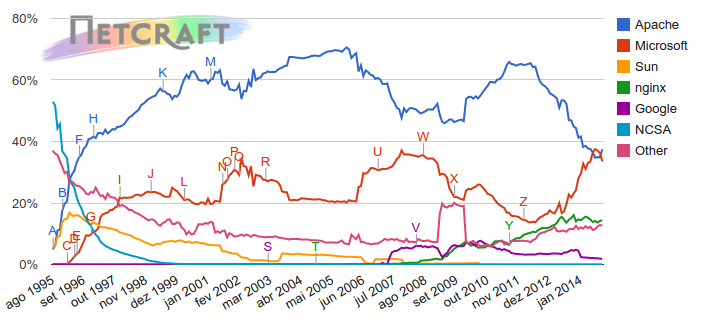
\includegraphics[width=1\linewidth]{figuras/grafico1}
	\caption{Utilização de Servidores \textit{web} no mundo.}
	\label{fig:webservers-utilizacao}
\end{figure}

\begin{figure}[htb]
	\centering
	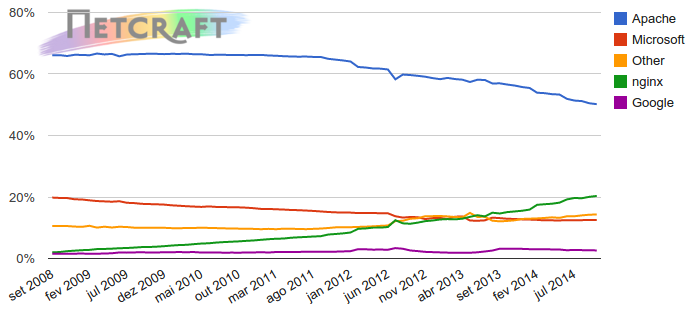
\includegraphics[width=1\linewidth]{figuras/grafico2} 
	\caption{Utilização de Servidores \textit{web} entre os 1.000.000 de sítios 
	mais acessados no mundo.}
	\label{fig:webservers-utilizacao-milhao}
\end{figure}

Ao analisar os gráficos apresentados nas figuras 
\ref{fig:webservers-utilizacao} e \ref{fig:webservers-utilizacao-milhao}, é 
possível notar uma queda na 
utilização do Apache em detrimento de outros servidores HTTP, sendo mais 
notória a queda na utilização entre 1 milhão de sítios mais acessados. É 
possível notar também o aumento no uso do Nginx, principalmente entre os 1 
milhão de sítios mais acessados no mundo. É necessário frisar que só porque uma 
tecnologia está em ascensão, não significa que ela é melhor, mas sim é 
necessário investigar os motivos pelos quais a tecnologia está crescendo em 
número de utilizadores.

Tendo sido desenvolvidos em épocas diferentes, o Apache e o Nginx trabalham de 
forma diferente na hora de atender as requisições HTTP que chegam ao servidor. 
De acordo com \citeonline{rowe}, o Apache cria processos e \textit{threads} 
para lidar com as requisições, ficando a cargo do administrador do servidor a 
tarefa de configurar o Apache para controlar o numero máximo de processos e 
\textit{threads} permitidos. Muitas \textit{threads} podem exaurir a memória 
principal(RAM) e pode forçar o servidor a usar memória \textit{SWAP}, 
degradando severamente o desempenho. Além disso, quando chega ao limite de 
processos, o Apache passa a recusar conexões.

\section{Motivação}
De acordo com o Plano de Desenvolvimento Institucional para o ciclo 2.012 - 
2.016 da UFVJM, além dos quatro \textit{campi} já implantados (Diamantina, 
Teófilo Otoni, Janaúba e Unaí), existe o projeto para a implantação de outros 
quatro \textit{campi} universitários nas cidade de Capelinha, Araçuaí, Almenara 
e Nanuque, totalizando oito \textit{campi} espalhados pelas regiões Norte, 
Noroeste, Vales do Jequitinhonha e Mucuri do estado de Minas Gerais. O 
PDI contempla também a ampliação da oferta de vagas e cursos de graduação 
nos já existentes \textit{campi} de Diamantina e Teófilo Otoni. Com a expansão 
das universidades federais através do programa REUNI, por ano são admitidos 
3500 alunos de graduação, pós-graduação e educação à distância além de novos 
servidores técnicos-administrativos e professores.

Em julho de 2.014, data do último levantamento, a Universidade Federal dos 
Vales do Jequitinhonha e Mucuri tinha 8.121 alunos, 576 professores e 421 
servidores técnicos-administrativos, espalhados em quatro \textit{campi} 
universitários, fazendas experimentais e pólos de ensino em educação à 
distância, totalizando 9.118 pessoas que interagem com a universidade 
diariamente. Em épocas de pico de utilização do SIGA, as reclamações de 
lentidão 
e problemas no SIGA são frequentes, as vezes impossibilitando a utilização do 
mesmo. Os picos mais notório são: fim de período letivo da graduação, quando 
alunos e professores acessam o sistema para olhar e lançar notas, 
respectivamente; e rematricula dos alunos da graduação, quando os mesmos 
escolhem as matérias que desejam cursar no período seguinte.

De acordo com dados retirados do registro de acesso da base de dados 
do SIGA, do dia 08 de Fevereiro de 2013, quando se começou a fazer esse 
registro, até o dia 27 de Novembro de 2.014, a data em que o SIGA obteve o 
maior número de acessos foi em 16 de Agosto de 2.014 com 20.942 acessos em 24 
horas, uma média de 873 registros de entrada por hora. O período de 9 à 10 
horas do dia 16/08 foi a hora com mais acessos da história com 1.351 
registros. Os dez dias com mais acessos ao SIGA estão representados na tabela 
\ref{tab:top10acessos}.

\begin{table}[htb]
	\centering
	\ABNTEXfontereduzida
	\caption{Dez dias com mais acessos no SIGA}
	\label{tab:top10acessos}
	\begin{tabular}{|c|c|c|}
		\hline
		\textbf{Dia} & \textbf{Acessos}  & \textbf{Ocasião} \\ \hline
		16/08/2014 & 20.942 & Início da Pré Matrícula \\ \hline
		25/08/2014 & 17.536 & Início do Período Letivo \\ \hline
		16/04/2013 & 17.091 & Dias Finais do Período Letivo \\ \hline
		30/09/2013 & 17.007 & Início da Pré Matrícula \\ \hline
		17/04/2013 & 16.772 & Dias Finais do Período Letivo \\ \hline
		15/04/2013 & 16.597 & Dias Finais do Período Letivo \\ \hline
		31/07/2014 & 16.035 & Dias Finais do Período Letivo \\ \hline
		29/07/2014 & 15.744 & Dias Finais do Período Letivo \\ \hline
		28/07/2014 & 15.477 & Dias Finais do Período Letivo \\ \hline
		30/07/2014 & 14.854 & Dias Finais do Período Letivo \\ \hline
	\end{tabular}
	\legend{Fonte: Base de Dados do SIGA}
\end{table}

Com o crescente aumento de alunos, servidores públicos (professores e 
técnicos-administrativos) e teceirizados na universidade, a tendência é que a 
utilização do SIGA se torne mais problemática.
Com isso em mente, a utilização do servidor HTTP Nginx pode ajudar a amenizar 
os problemas de desempenho do SIGA.

\section{Objetivos}

Identificar se a utilização do servidor HTTP Nginx é mais eficiente do que o 
utilizado atualmente, o Apache HTTP \textit{Server}.

\section{Objetivos específicos}

Analisar os dados coletados a partir de testes realizados para identificar se o 
Nginx é mais eficiente do que o Apache; apresentar a solução encontrada e 
analisar o que pode ser feito para evitar a substituição ou reconstrução do 
SIGA.

\section{Organização do trabalho}
O trabalho está organizado em seis capítulos, sendo essa introdução o primeiro. 
No capítulo \ref{cap:fundamentacao-teorica}, será exposto toda a teoria por 
trás do estudo feito. No capítulo \ref{cap:tecnologias_utilizadas}, serão 
descritos os programas e ferramentas utilizados de forma direta ou indireta nos 
testes. No capítulo \ref{cap:metodologia} será descrito como os testes foram 
realizados, quais dados foram coletados e descrever os ambientes onde foram 
feitos os teste de desempenho do Apache e do Nginx. No capítulo 
\ref{cap:analise-dos-dados} os dados serão apresentados e 
será feita uma análise sobre o desempenho dos dois servidores HTTP. E 
finalmente, no capítulo \ref{cap:conclusao} será apresentada uma conclusão 
sobre o estudo.
